\documentclass{article}

\usepackage{graphicx}
\usepackage{tikz}
\usepackage{tikzsymbols}
\usetikzlibrary{calc,patterns,shapes.geometric}
\pagestyle{empty}
\usepackage[margin=0pt]{geometry}
\geometry{papersize={14in,12in}}

\def\centerarc[#1](#2)(#3:#4:#5){\draw[#1] ($(#2)+({#5*cos(#3)},{#5*sin(#3)})$) arc (#3:#4:#5);}

\begin{document}
	\begin{figure}
		\centering
		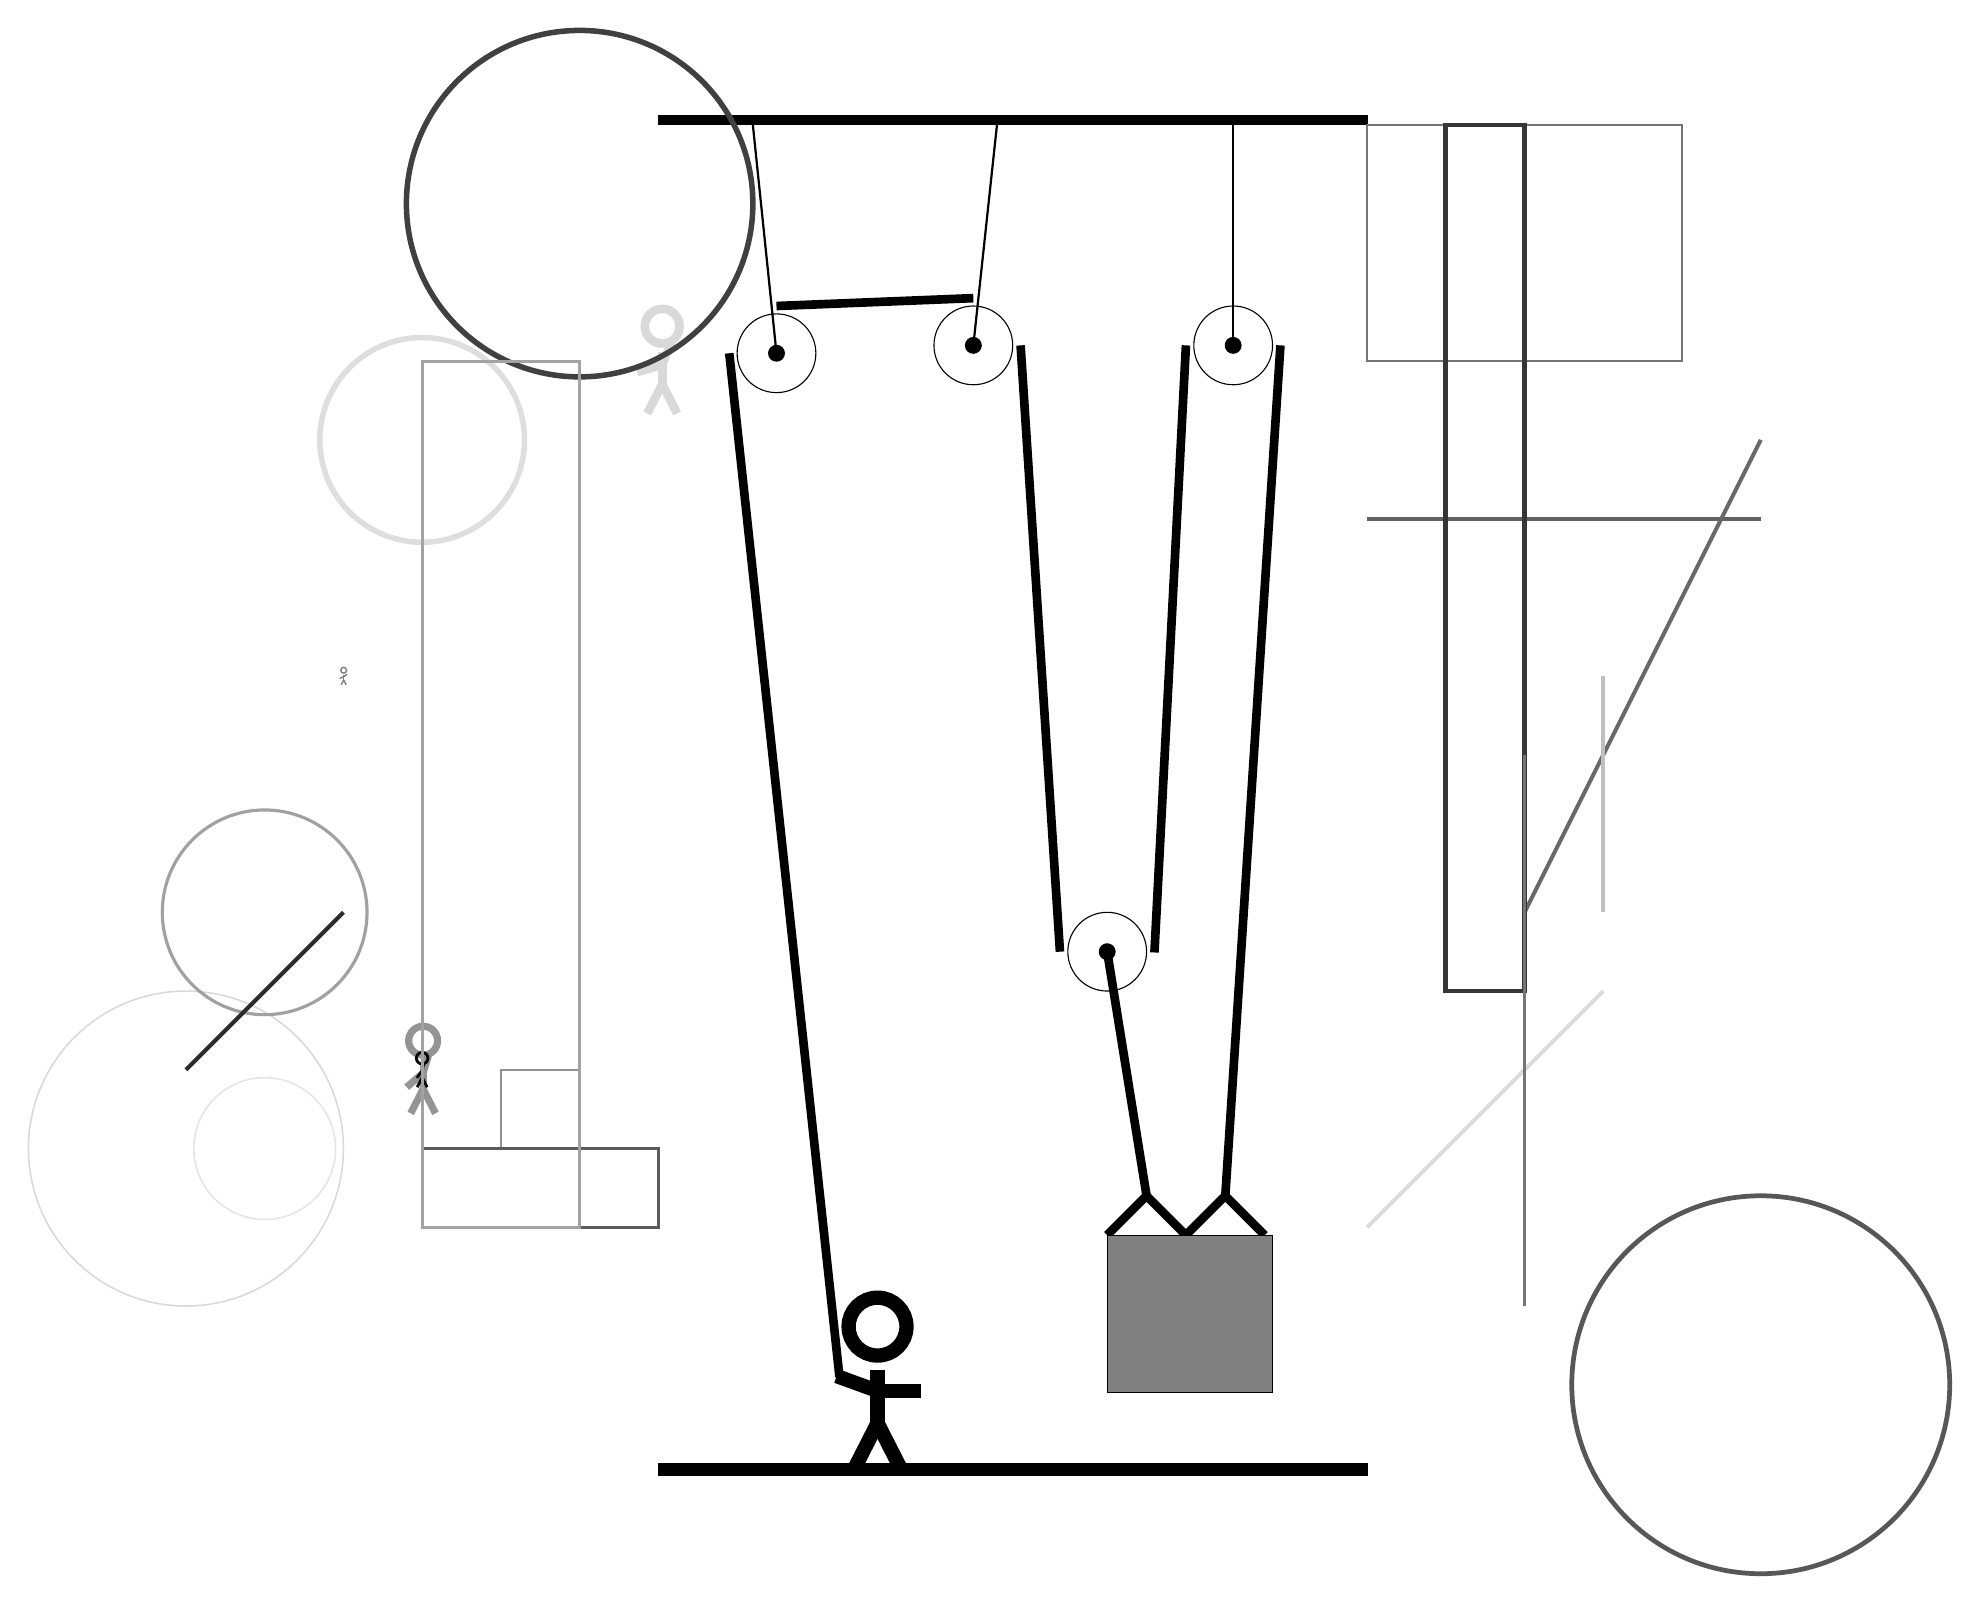
\begin{tikzpicture}
			%%%%% START %%%%%
			
			\draw[fill=black] (-3, 14) rectangle (6, 14.125);
			
			\draw (1, 11.2) circle (0.5);
			\draw[fill=black] (1, 11.2) circle (0.1);
			\draw[thick] (1, 11.2) -- (1.3, 14);
			
			\draw (4.3, 11.2) circle (0.5);
			\draw[fill=black] (4.3, 11.2) circle (0.1);
			\draw[thick] (4.3, 11.2) -- (4.3, 14);
			
			\draw [line width=0.2mm, color=black!15](-9, 1) circle (2.0);
			
			\node[line width=0.6mm, color=black!15] at (-3, 11) {\Strichmaxerl[6][16][68]};
			\draw[line width=0.5mm, color=black!62](6, 9) -- (11, 9);
			\draw [line width=0.6mm, color=black!66](11, -2) circle (2.4);
			
			\draw[line width=0.3mm, color=black!44] (-5, 1) rectangle (-4, 2);
			\draw[line width=0.5mm, color=black!59](11, 10) -- (8, 4);
			
			\draw [line width=0.4mm, color=black!37](-8, 4) circle (1.3);
			\draw[line width=0.3mm, color=black!54] (6, 14) rectangle (10, 11);
			\draw[line width=0.6mm, color=black!79] (7, 14) rectangle (8, 3);
			\draw [line width=0.7mm, color=black!75](-4, 13) circle (2.2);
			
			\draw[line width=0.5mm, color=black!83](-7, 4) -- (-9, 2);
			\node[line width=0.3mm, color=black!50] at (-7, 7) {\Strichmaxerl[1][23][36]};
			\draw [line width=0.2mm, color=black!10](-8, 1) circle (0.9);
			
			\draw[line width=0.5mm, color=black!14](9, 3) -- (6, 0);
			\draw[line width=0.4mm, color=black!64] (-3, 0) rectangle (-6, 1);
			\draw [line width=0.7mm, color=black!13](-6, 10) circle (1.3);
			\node[line width=0.3mm, color=black!42] at (-6, 2) {\Strichmaxerl[5][41][73]};
			\node[line width=0.7mm, color=black!96] at (-6, 2) {\Strichmaxerl[2][52][78]};
			\draw[line width=0.5mm, color=black!25](9, 7) -- (9, 4);
			
			\draw[line width=0.4mm, color=black!54] (8, -1) rectangle (8, 6);
			\draw[line width=0.4mm, color=black!36] (-4, 11) rectangle (-6, 0);
			
			
			\draw (2.7, 3.5) circle (0.5);
			\draw[fill=black] (2.7, 3.5) circle (0.1);
			
			\draw[line width=1.1mm]  (2.7, -0.1) -- (3.2, 0.4) -- (3.7, -0.1) -- (4.2, 0.4) -- (4.7, -0.1);
			\draw[fill=black!50] (2.7, -0.1) rectangle (4.8, -2.1);
			
			\draw (-1.5, 11.1) circle (0.5);
			\draw[fill=black] (-1.5, 11.1) circle (0.1);
			\draw[thick] (-1.5, 11.1) -- (-1.8, 14);
			
			\draw[line width=1.1mm](-0.7, -1.9) --  (-2.1, 11.1);
			\centerarc[line width=1.1mm](-1.5, 11.1)(90:180:0.6);
			\draw[line width=1.1mm](-1.5, 11.7) -- (1, 11.8);
			\centerarc[line width=1.1mm](1, 11.2)(0:90:0.6);
			\draw[line width=1.1mm](1.6, 11.2) -- (2.1, 3.5);
			\centerarc[line width=1.1mm](2.7, 3.5)(180:370:0.6);
			\draw[line width=1.1mm] (3.3, 3.49) -- (3.7, 11.2);
			\centerarc[line width=1.1mm](4.3, 11.2)(0:180:0.6);
			\draw[line width=1.1mm](4.2, 0.4) -- (4.9, 11.2);
			\draw[line width=1.1mm] (3.2, 0.4) -- (2.7, 3.5);
			
			\node at (-0.2, -2) {\Strichmaxerl[10][-20][0]};
			
			\draw[fill=black] (-3, -3) rectangle (6, -3.15);
			
			%%%%% END %%%%%
		\end{tikzpicture}
	\end{figure}	
\end{document}